% main.tex — IEEEtran (LuaLaTeX, luatexja)
% Build: lualatex main.tex ; lualatex main.tex
\documentclass[conference]{IEEEtran}

% ---- Japanese (LuaLaTeX) ----
\usepackage{luatexja}
\usepackage{luatexja-fontspec}
% フォントはTeXLive同梱の原ノ味で安全
\setmainjfont{HaranoAjiMincho}
\setsansjfont{HaranoAjiGothic}

% ---- General packages (IEEE互換の範囲) ----
\usepackage{siunitx}
\sisetup{mode=match,propagate-math-font=true}
\usepackage{graphicx}
\usepackage{xcolor}
\usepackage{booktabs}
\usepackage{cite}      % 参考文献の整形(使わなければ外してOK)
\usepackage[hidelinks]{hyperref}

% ---- TikZ(図は本文内に埋め込み)----
\usepackage{tikz}
\usetikzlibrary{arrows.meta,calc}

% ====== 内蔵図コマンド ======
% ドーナツ状のボイド分布
\newcommand{\figVoidDonutInline}{%
  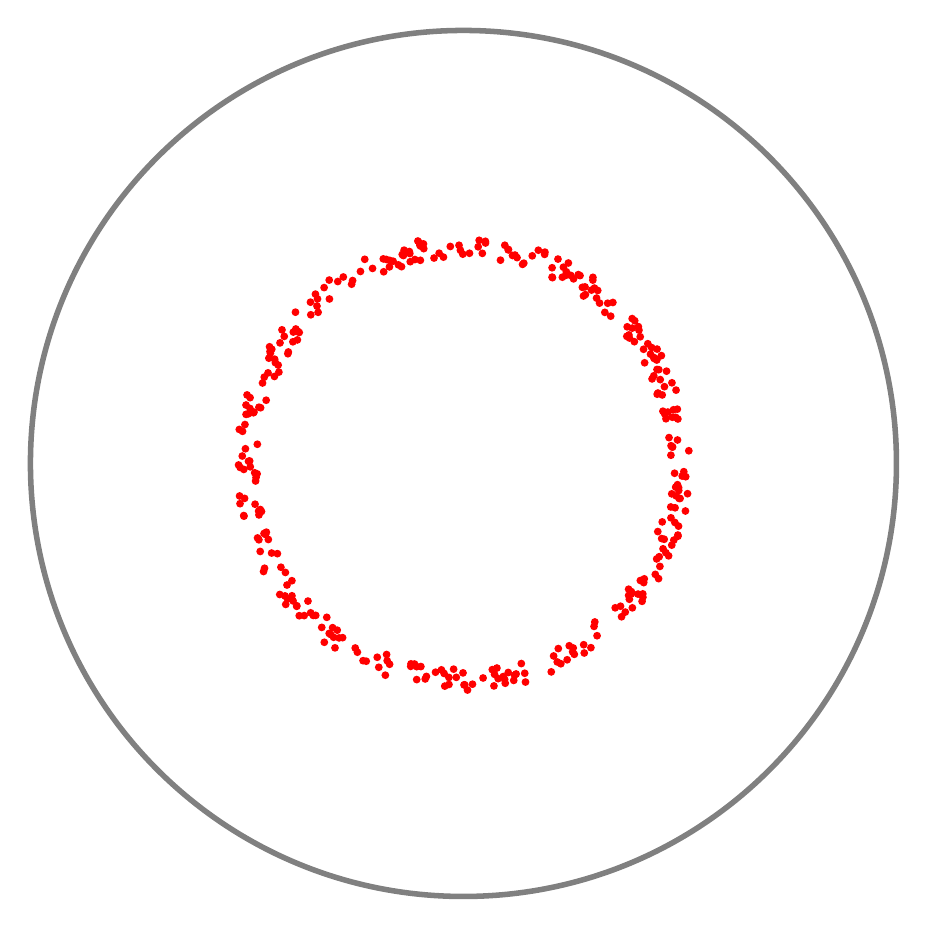
\begin{tikzpicture}[scale=0.055]
    \draw[line width=2pt, gray] (0,0) circle (100);
    \foreach \i in {1,...,360}{%
      \pgfmathsetmacro{\ang}{rnd*360}
      \pgfmathsetmacro{\rad}{50 + 5*(rnd-0.5)}
      \fill[red] (\ang:\rad) circle (0.9);
    }
  \end{tikzpicture}%
}

% 6層中1層にボイド(矩形)を含む断面
\newcommand{\figPZTLayersVoidInline}{%
  \begin{tikzpicture}[x=0.9cm,y=0.9cm]
    \def\W{6.0}\def\H{0.45}\def\G{0.10}
    \foreach \i in {0,...,5}{
      \pgfmathsetmacro{\y}{\i*(\H+\G)}
      \draw[fill=gray!20,draw=black] (0,\y) rectangle (\W,\y+\H);
    }
    % 第4層のボイド
    \pgfmathsetmacro{\yv}{3*(\H+\G)}
    \draw[very thick,red] (2.1,\yv+0.08) rectangle (3.0,\yv+\H-0.08);
    % 上下のリファレンス線(電極イメージ)
    \draw[line width=1pt] (0,-0.30) -- (\W,-0.30);
    \draw[line width=1pt] (0,6*(\H+\G)+0.10) -- (\W,6*(\H+\G)+0.10);
  \end{tikzpicture}%
}

% 端部焼損の模式(カラー)
\newcommand{\figEdgeBurnoutInline}{%
  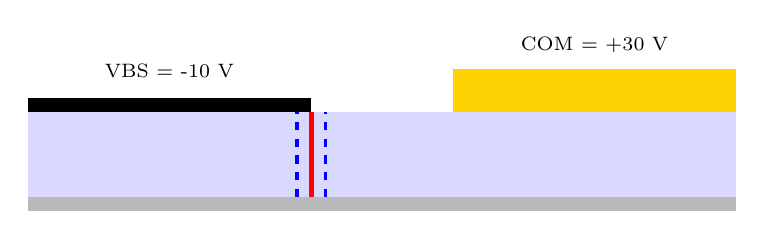
\begin{tikzpicture}[x=0.9cm,y=0.9cm]
    \def\W{10}\def\pztH{1.2}\def\beH{0.20}\def\teH{0.20}
    % Bottom Electrode (BE)
    \fill[gray!55] (0,0) rectangle (\W,\beH);
    % PZT layer
    \fill[blue!15] (0,\beH) rectangle (\W,\beH+\pztH);
    % Top Electrode = VBS
    \fill[black] (0,\beH+\pztH) rectangle (4,\beH+\pztH+\teH);
    % Au pad = COM
    \fill[yellow!70!orange] (6,\beH+\pztH) rectangle (\W,\beH+\pztH+0.60);
    % Exposed sidewall (electric field focus)
    \draw[line width=1.8pt,red] (4,\beH) -- (4,\beH+\pztH);
    % Proposed AlOx (ALD)
    \draw[line width=1.2pt,blue,dashed] (3.8,\beH) -- (3.8,\beH+\pztH);
    \draw[line width=1.2pt,blue,dashed] (4.2,\beH) -- (4.2,\beH+\pztH);
    % Labels
    \node[anchor=south] at (2, \beH+\pztH+\teH+0.15) {\scriptsize VBS = -10 V};
    \node[anchor=south] at (8, \beH+\pztH+0.70) {\scriptsize COM = +30 V};
  \end{tikzpicture}%
}

% ====== タイトル/著者 ======
\title{PZT薄膜アクチュエータにおける振動板クラックと端部焼損の原因解析・対策提案}

\author{%
  \IEEEauthorblockN{Shinichi Samizo}
  \IEEEauthorblockA{Independent Semiconductor Researcher\\
  Former Engineer at Seiko Epson Corporation\\
  Email: \href{mailto:shin3t72@gmail.com}{shin3t72@gmail.com} \quad
  GitHub: \url{https://github.com/Samizo-AITL}}
}

\begin{document}
\maketitle

\begin{abstract}
Epson $\mu$TFP(薄膜PZT $d_{33}$)アクチュエータで観測された
(1) 振動板クラック、(2) セグメント端部焼損について、原因解析と対策を示す。
クラックはRTA後の表面疎水化が起点となりスピン塗布で気泡を巻き込み膜内ボイド化。
酢酸プレウェット導入で不良率を5--10\%から$\approx$0\%へ低減した。
焼損はCOM--VBS近接端部での電界集中(\SI{40}{V}差、台形波立上り)による局所絶縁破壊が主因と推定し、
ALD--AlOx被覆を提案する。
\end{abstract}

\begin{IEEEkeywords}
Inkjet, PrecisionCore ($\mu$TFP), Thin-film PZT, $d_{33}$ mode, Reliability, Crack, Edge Burnout
\end{IEEEkeywords}

\section{序論}
Mach(バルク積層PZT, $d_{31}$, 180\,dpi)から薄膜PZT TFP/$\mu$TFP($d_{33}$, 300\,dpi)への移行により
高密度・高応答化を実現した一方、薄膜特有の欠陥感受性と高電界条件下で
クラック/端部焼損が顕在化した。本稿は量産工程で遭遇した両事象の解析と対策を要約する。

\section{デバイス・プロセス構成}
PZTはゾルゲル法による\SI{200}{nm}$\times6$(総\SI{1.2}{\micro m})。
第1層焼成後にTi \SI{4}{nm}を挿入し組成傾斜を緩和。
下電極はPt(111)/Ir seed,上電極はIr/Ti。ドライバICはCMOS \SI{0.35}{\micro m},
\SI{3.3}{V}/\SI{45}{V},400ch$\times$2列。

\section{結果}
\subsection{クラック:同心リング分布と層内ボイド}
長期放置後の塗布・焼成ロットで、反射条件最適化の検査により
半径中間域にドーナツ状の欠陥分布を検出(Fig.~\ref{fig:donut})。
断面観察では6層中の特定層にボイドが局在(Fig.~\ref{fig:layer-void})。

\begin{figure}[t]
  \centering
  \figVoidDonutInline
  \caption{ウエハ上のドーナツ状ボイド分布(反射条件最適化)}
  \label{fig:donut}
\end{figure}

\begin{figure}[t]
  \centering
  \figPZTLayersVoidInline
  \caption{PZT 6層のうち1層にボイドを含む断面模式図}
  \label{fig:layer-void}
\end{figure}

\subsection{端部焼損:電界集中部位}
ユニットスクリーニング(DC 60\,s, AC 90\,s, COM +\SI{30}{V}, VBS \SI{-10}{V}, 台形波)で
COM(Au配線)とVBS(上電極)が最接近する側壁露出部に焼損(Fig.~\ref{fig:edge})。
差分\SI{40}{V}での立上り瞬間電流が重畳し局所絶縁破壊を誘発。

\begin{figure}[t]
  \centering
  \figEdgeBurnoutInline
  \caption{端部焼損の模式図(電界集中部とAlOx対策案)}
  \label{fig:edge}
\end{figure}

\section{考察}
\textbf{クラック:} RTA後の外気由来付着でPZT表面が疎水化し、スピン時に気泡を巻き込み→膜内ボイド化。
暫定的にロードロック防壁、恒久的に酢酸プレウェットを導入。XRD配向率、ヒステリシス、吐出特性で
従来条件との差は有意差なし。

\textbf{焼損:} 構造上避け難い側壁露出+高電位差で電界集中。対策案としてALD--AlOx端部被覆、
電圧マージン緩和(例:+\SI{25}{V}/\SI{-5}{V})や版下改良を提示。

\section{結論}
クラックは酢酸プレウェット導入で5--10\%からほぼ0\%へ撲滅。焼損は原因を特定し、
AlOx被覆を主案として提案した。薄膜PZT $d_{33}$方式の量産信頼性向上に資する。

\section*{Author Biography}
\textbf{Shinichi Samizo} received the M.S. degree in Electrical and Electronic
Engineering from Shinshu University, Japan. He worked at Seiko Epson Corporation
on semiconductor and inkjet MEMS (PrecisionCore). He is currently an independent
semiconductor researcher. Contact: \href{mailto:shin3t72@gmail.com}{shin3t72@gmail.com}.

\end{document}
